% =========================  
% Seções/1-Introdução.tex  
% (não usar \section{Introdução} aqui;  
%  o capítulo é aberto no main.tex)  
% =========================  
  
A resolução de problemas por \emph{busca} ocupa posição central na Inteligência Artificial (IA) simbólica: modela a navegação em um \emph{espaço de estados} por meio de operadores, avaliando custos e selecionando expansões segundo políticas informadas ou não informadas, como discutem \citeonline{russell2010artificial} e \citeonline{nilsson1998}. O interesse central está em compreender como diferentes algoritmos percorrem esse espaço, quais estruturas de dados utilizam e de que modo heurísticas afetam o desempenho.  
  
Para fins experimentais, optou-se pelo \emph{8-puzzle} como domínio de teste. Trata-se de um tabuleiro $3\times 3$ com oito peças móveis e um espaço vazio, cujo objetivo é atingir uma configuração final a partir de um arranjo inicial (Figura~\ref{fig:8puzzle}).   
  
\begin{figure}[H]  
    \centering  
    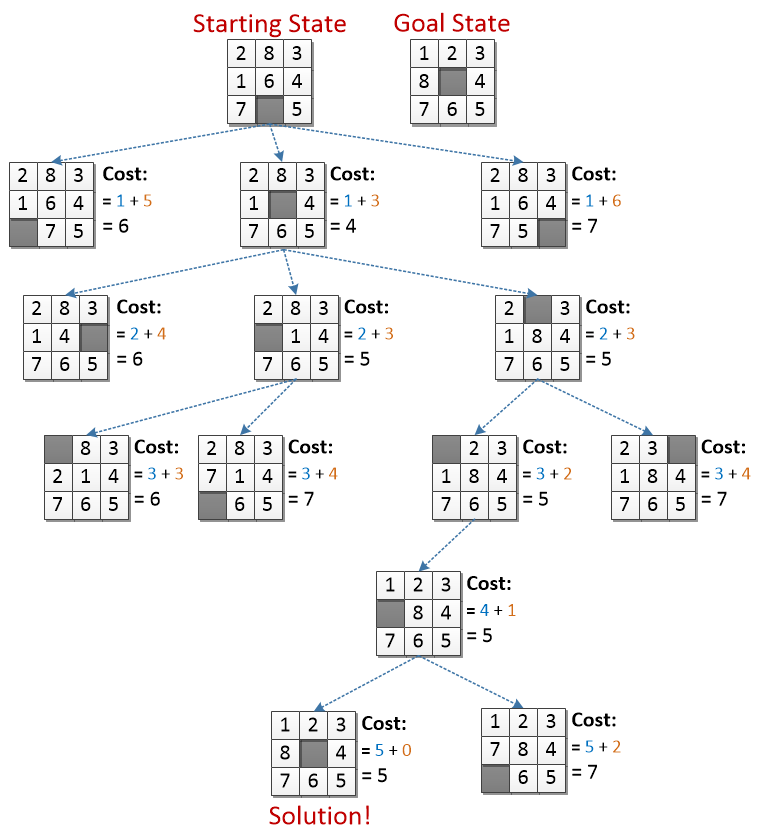
\includegraphics[width=0.8\textwidth]{Imagens/8puzzle7.png}  
    \caption{Exemplo de estados do problema do 8-puzzle, com estado inicial, transições e estado objetivo.}  
    \caption*{\textit{Fonte: elaborado pelos autores.}}  
    \label{fig:8puzzle}  
\end{figure}  
  
A escolha deste problema não se deve à sua complexidade prática, mas sim por ser computacionalmente leve, o que permite implementar e comparar variações de algoritmos de busca de forma controlada e reprodutível. Assim, o foco da análise permanece nos métodos de busca --- custo uniforme e versões do algoritmo $A^*$ com heurísticas de diferentes níveis de admissibilidade --- e não no quebra-cabeça em si. Nesse contexto, o 8-puzzle funciona como um \emph{laboratório didático} que viabiliza a avaliação sistemática de desempenho.  
  
No âmbito da disciplina INE5633---\emph{Sistemas Inteligentes} (UFSC), esta Atividade Prática 1 (AP1) utiliza o 8-puzzle como laboratório para implementar e analisar o algoritmo $A^*$ e suas variações, em alinhamento ao conteúdo de \emph{raciocínio e resolução de problemas} e à ênfase em técnicas de busca e informação heurística. A proposta didática privilegia a implementação e análise prática, conforme a bibliografia básica adotada \cite{russell2010artificial,luger2009artificial}.  
  
\vspace{0.5cm}  
\section{Escopo desta Atividade Prática}  
  
Serão estudadas quatro variantes:  
\begin{enumerate}[label=\roman*)]  
  \item Busca de custo uniforme (sem heurística);  
  \item $A^*$ com heurística \emph{não admissível};  
  \item $A^*$ com heurística admissível simples;  
  \item $A^*$ com a heurística admissível mais precisa desenvolvida pela equipe.  
\end{enumerate}  
  
A comparação considerará:  
\begin{itemize}  
  \item Total de nós visitados;  
  \item Comprimento do caminho-solução;  
  \item Maior tamanho da fronteira (abertos);  
  \item Tempo de execução;  
  \item Geração de arquivo \texttt{.txt}/\texttt{.json} com fronteira e visitados ao término.  
\end{itemize}  
  
Esses indicadores permitem discutir \emph{admissibilidade} e \emph{consistência} das heurísticas no $A^*$, além de seus efeitos na eficiência \cite{russell2010artificial,luger2009artificial}.  
  
\vspace{0.5cm}  
\section{Objetivos formativos}  
  
Consolidar, por meio de implementação e experimentação reprodutível, a ponte entre teoria e prática em busca. Em particular, pretende-se:  
\begin{enumerate}[label=(\alph*),leftmargin=*,itemsep=0pt,topsep=2pt]  
  \item Formalizar o problema como \emph{espaço de estados} (definição de estados, operadores, teste de objetivo e função de custo);  
  \item Projetar e gerir a \emph{fronteira}, com checagem de dominância e de estados repetidos (políticas de inserção/remoção e estrutura de dados apropriada);  
  \item Definir e justificar heurísticas (admissíveis e não admissíveis), discutindo propriedades como admissibilidade e consistência;  
  \item Analisar comparativamente o desempenho das variantes (UCS e $A^*$), com métricas reprodutíveis e interpretação crítica.  
\end{enumerate}  
A fundamentação teórica apoia-se em \citeonline{russell2010artificial,nilsson1998} e obras complementares como \citeonline{ertel2017}.  
  
\vspace{0.5cm}  
\section{Contribuições esperadas}  
  
O relatório apresentará:  
\begin{enumerate}[label=(\roman*),leftmargin=*,itemsep=0pt,topsep=2pt]  
  \item A modelagem do 8-puzzle e as estruturas de dados utilizadas;  
  \item O $A^*$ e o UCS com suas políticas de fronteira e critérios de expansão;  
  \item O desenho das heurísticas, com justificativa matemática e discussão sobre admissibilidade/consistência;  
  \item A avaliação experimental (casos fáceis, médios e difíceis), com comparação de nós visitados, comprimento do caminho-solução, maior tamanho da fronteira, tempo de execução e arquivo \texttt{.txt}/\texttt{.json} contendo fronteira e visitados ao término.  
\end{enumerate}  
A análise será fundamentada na literatura clássica \cite{russell2010artificial,luger2009artificial,nilsson1998,ertel2017} e será reprodutível a partir dos artefatos entregues (código e logs).  